\chapter{Introduction}
\emph{The chapter starts with a background describing why road condition monitoring is important and who Trafikverket are, how road condition data is collected today and why the technology behind it needs improvement. An objective for the project is defined followed by its delimitations. Lastly, a thesis structure is presented to simplify navigation through different parts of the project.}

\section{Background} \label{sec:background}
	Living in cold areas of the world usually means work for invididual people, municipalities and companies in trying to maintain a non-winter-like infrastructure. This of course, also involves winter road maintenance. Salting and plowing roads is an investment in not only saving lives, but also in lowering socio-economic costs: In two scenarios on a road with 2 cm snow and a daily traffic flow of 2000 vehicles, one with a salted and ploughed road taking four hours to drive, and another scenario on the same road without winter maintenance taking five hours to drive. The total socio-economic costs are 3.5\% higher in the non-maintained road, mainly due to increased travel time and thus higher accident costs \cite{ARTICLE:1}. 

	Despite the socio-economic savings in performing winter road maintenance, it still represents a notable economic cost. Trafikverket, the agency in charge of road state road maintenance in Sweden, reported that winter road maintenance were roughly 18\% of the total road maintenance costs in 2013 \cite{REPORT:1}. Local contracters are hired to carry out the plowing and salting of state roads, with requirements on both ends regarding when to plow, which roads to prioritize etc. Trafikverket has over 800 Road Weather Information Systems (RWIS)(Fig. \ref{img:rwis}) distributed across state roads in Sweden which are used by contracters to carry out winter road maintenance work \cite{WEBSITE:2}. 
\begin{figure}[H]
	\centering
	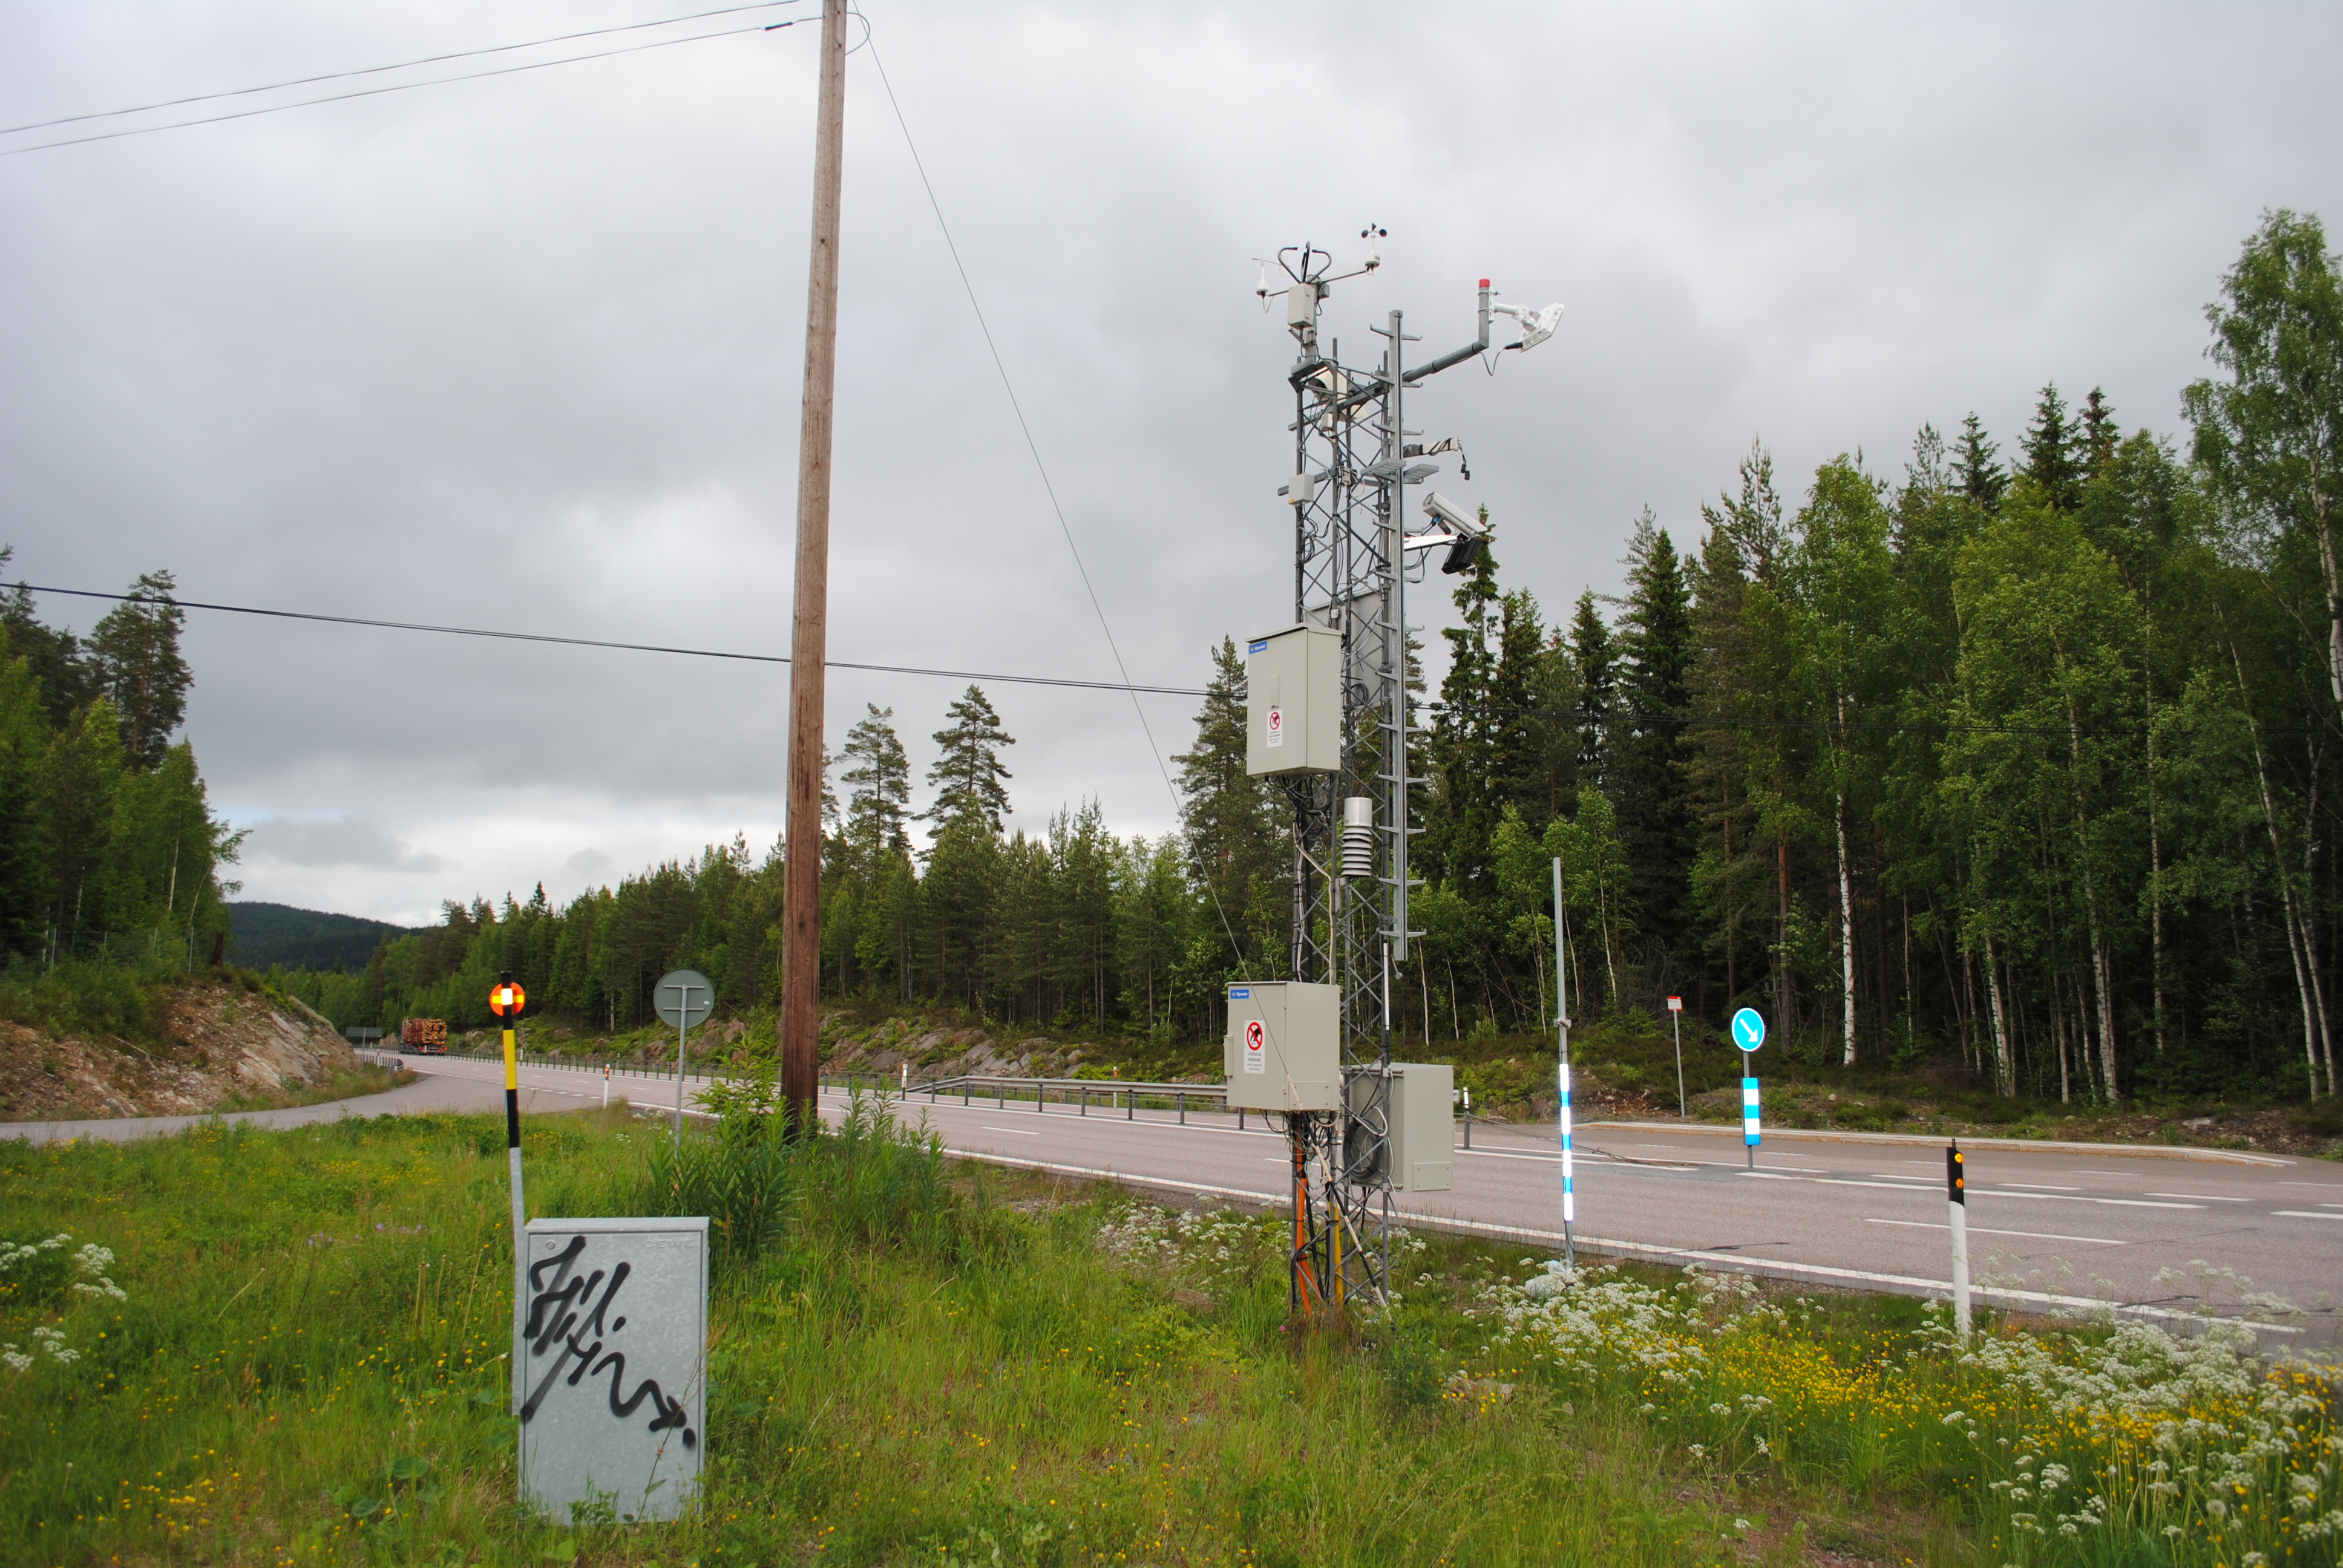
\includegraphics[width=0.8\textwidth]{media/Rwis_station_Myggsjon_01.JPG}
	\caption{RWIS Station at sensor site Myggsjön \cite{IMAGE:1}.}
	\label{img:rwis}
\end{figure}

	The RWIS show different information depending on what instruments they have, %but in 80% of the RWIS they have the following informationTable \ref{table:rwis} shows 

\begin{tabular}[3]{c | c | c}
    	Operation & worst-case cost & time complexity \\
    	\hline
    	Insert $x$ into $l_i$ & 2 & $O(1)$  \\
   	Update $count_i$ & 1 &$O(1)$ \\
	\label{table:rwis}
\end{tabular}

	%problems with sensors
	%which tools can be used to model sensors? machine learning, statistical tools
	%why machine learning?

	Machine learning as formally defined by Mitchell \cite{BOOK:2}: 
"A computer program is said to learn from experience $E$ with respect to some class of tasks $T$ and performance measure $P$ if its performance at tasks in $T$, as measured by $P$, improves with experience $E$".	This means that machine learning algorithms are used to solve a set of problems, measure its performance in doing so and ultimately improve in some way from previous experiences. For example, imagine a program designed to determine if a human face is in a photo or not. Since photos are taken at different distances, angles and faces have different characteristics such as eye color, skin color, distance between eyes and nose shape, implementing this "manually" may prove cumbersome. Instead of programming an algorithm to recognize faces, it can be programmed  \emph{to learn to recognize faces}. If the algorithm is allowed to analyze a dataset with thousands of photos of human faces, it could learn to distinguish a human face by recognizing parts of the face such as eyes, nose, mouth and where those parts are most likely placed to oneanother.

	In essence, machine learning algorithms improve/learn in some way from analyzing a dataset. How they learn can be used to broadly categorize machine learning algorithms as either having supervised or unsupervised learning \cite{BOOK:1}. Supervised learning algorithms processes a labeled dataset while unsupervised learning attempts to make sense of unlabeled data \cite{BOOK:3}. For that reason, it makes sense to see which of the RWIS sensors can be modelled using supervised learning algorithms.

%why not use all features? 
%1. CURSE OF DIMENSIONALITY @ebook, " The basic premise of the curse of dimensionality is that high dimensional data brings in complexity. With more dimensions and features, the possibility of errors is also high"
%2. johan casselgrens argument

%which machine learning algorithm? hard! explain why different algorithms are compared and why scikit learn is used for this.


\section{Objective}
	The objective is to find which supervised learning algorithms that best models MS-4 surface temperature, precipitation type and precipitation amount by building and comparing supervised learning models available in Scikit-learn. The models are built from data provided by six weather stations along state road e6 with 171425 observations over two years measuring the following every 30 minutes: MS4 surface temperature, MS4 Precipitation type, MS4 Precipitation amount, DST111 surface temperature, DSC111 friction, DSC111 surface type.  %define "best" 

\section{Delimitations} \label{sec:delimitations}
	There are many supervised learning algorithms, all of which are not evaluated in detail in this project. An algorithm is qualified for evaluation in this project if the following is true:
	\begin{enumerate}
		\item The algorithm is a supervised learning algorithm that solves regression and/or multiclass classification problems (see \ref{sec:classification} and \ref{sec:regression})
		\item The algorithm is available in Scikit-learn \cite{WEBSITE:15}
		\item The algorithm belongs to one of the following algorithm families (see \ref{sec:supervised_algorithms}):
			\begin{itemize}
				\item Decision tree based learning %cart
				\item Instance based learning %knn
				%\item Kernel methods based learning %svm
				\item Bayesian learning %GaussianNB
				\item Regression based learning %linear regression, logistic regression, lasso?
				\item Deep learning %backpropagation
				\item Ensemble learning %random forest
			\end{itemize}
	\end{enumerate}
	At least one algorithm per family, as listed above, are evaluated in this project. The reason for this is that algorithms from same families generally perform well on similar situations. %need cite
Only linear algorithms are considered from Regression based learning algorithms. The reason for limiting this family to linear algorithms is because every other algorithm in the other families, except for Naïve bayes, are considered nonlinear, and are thus overrepresented in the project. 
	
\section{Thesis structure}
% explain what the thesis looks like
